% A product rectangle and a triangle, with one vertical slice and one horizontal slice.
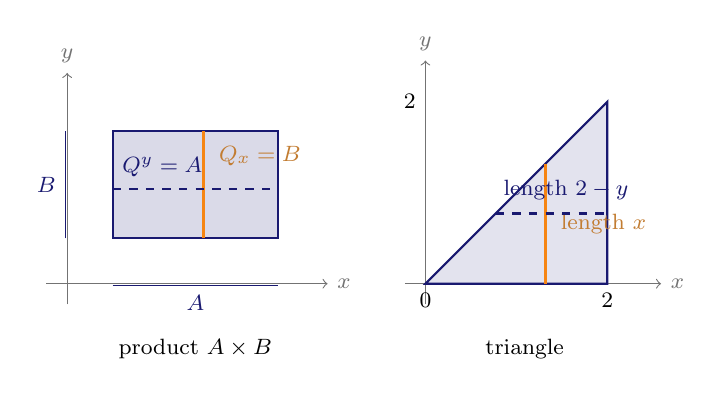
\begin{tikzpicture}[x=1.05cm,y=1.05cm,every node/.style={font=\footnotesize}]
  % Left: the rectangle A times B.
  \draw[->,black!55] (-0.25,0) -- (3.15,0) node[right] {$x$};
  \draw[->,black!55] (0,-0.25) -- (0,2.55) node[above] {$y$};
  \fill[MidnightBlue!16] (0.55,0.55) rectangle (2.55,1.85);
  \draw[MidnightBlue,thick] (0.55,0.55) rectangle (2.55,1.85);
  \draw[BurntOrange,very thick] (1.65,0.55) -- (1.65,1.85);
  \node[BurntOrange!75!black,anchor=west] at (1.72,1.55) {$Q_x=B$};
  \draw[MidnightBlue,thick,dashed] (0.55,1.15) -- (2.55,1.15);
  \node[MidnightBlue,anchor=south] at (1.15,1.18) {$Q^y=A$};
  \draw[MidnightBlue] (0.55,-0.02) -- (2.55,-0.02);
  \node[MidnightBlue,below] at (1.55,-0.02) {$A$};
  \draw[MidnightBlue] (-0.02,0.55) -- (-0.02,1.85);
  \node[MidnightBlue,left] at (-0.02,1.2) {$B$};
  \node[anchor=north] at (1.55,-0.55) {product $A\times B$};
  % Right: a triangle that is not a rectangle.
  \begin{scope}[xshift=4.55cm]
    \draw[->,black!55] (-0.25,0) -- (2.85,0) node[right] {$x$};
    \draw[->,black!55] (0,-0.25) -- (0,2.7) node[above] {$y$};
    \fill[MidnightBlue!12] (0,0) -- (2.2,0) -- (2.2,2.2) -- cycle;
    \draw[MidnightBlue,thick] (0,0) -- (2.2,0) -- (2.2,2.2) -- cycle;
    \draw[BurntOrange,very thick] (1.45,0) -- (1.45,1.45);
    \node[BurntOrange!75!black,anchor=west] at (1.52,0.72) {length $x$};
    \draw[MidnightBlue,thick,dashed] (0.85,0.85) -- (2.2,0.85);
    \node[MidnightBlue,anchor=south] at (1.7,0.9) {length $2-y$};
    \node[below] at (0,0) {$0$};
    \node[below] at (2.2,0) {$2$};
    \node[left] at (0,2.2) {$2$};
    \node[anchor=north] at (1.2,-0.55) {triangle};
  \end{scope}
\end{tikzpicture}
